\documentclass[10pt, xcolor={table}]{beamer}
\usepackage[]{graphicx}
\usepackage[]{color}


\AtBeginDocument{\abovedisplayshortskip=10pt plus 3pt}
\AtBeginDocument{\belowdisplayshortskip=20pt plus 3pt minus 4pt}

%% maxwidth is the original width if it is less than linewidth
%% otherwise use linewidth (to make sure the graphics do not exceed the margin)
\makeatletter
\def\maxwidth{ %
  \ifdim\Gin@nat@width>\linewidth
    \linewidth
  \else
    \Gin@nat@width
  \fi
}
\makeatother

\usepackage{listings}


\newcommand{\backupbegin}{
   \newcounter{framenumberappendix}
   \setcounter{framenumberappendix}{\value{framenumber}}
}
\newcommand{\backupend}{
   \addtocounter{framenumberappendix}{-\value{framenumber}}
   \addtocounter{framenumber}{\value{framenumberappendix}} 
}



\usepackage{alltt}

\usepackage{url,verbatim}
\usepackage[english]{babel}

\usepackage{avant}
\renewcommand*\familydefault{\sfdefault} %% Only if the base font of the document is to be sans serif
\usepackage[T1]{fontenc}

\usepackage{tikz}
\usetikzlibrary{positioning,shapes,arrows,decorations.pathreplacing,calc,automata}
\usepackage{pgfplots}
\pgfplotsset{compat=1.10}
\usepackage{calc}
% load extra stuff
% \usetikzlibrary{shapes.misc,matrix,positioning,fit}

% cross out text 
\usepackage[normalem]{ulem}


\usepackage[headheight=22pt]{beamerthemeboxes}
%\usepackage{bbm}
\usepackage{graphicx}
\beamertemplatenavigationsymbolsempty 
\setbeamercovered{transparent}

% \definecolor{redve}{rgb}{0.604,0.008,0.00}
\definecolor{redve}{rgb}{0,0.61,0.245}
% \definecolor{uzh}{rgb}{0.188,0.522,0.306}
\definecolor{uzh}{HTML}{0028a5}
\setbeamertemplate{itemize item}{$\bullet$} 
\setbeamercolor{title}{fg=uzh}
\setbeamercolor{frametitle}{fg=uzh}
\setbeamertemplate{sections/subsections in toc}[ball unnumbered]
\setbeamercolor{section in toc}{fg=uzh,bg=white}
\setbeamercolor{subsection in toc}{fg=uzh,bg=white}
\setbeamercolor{result}{fg=black, bg=yellow}



% \addheadboxtemplate{\color[rgb]{1,1,1}}{\color{uzh} \underline{\hspace{10cm} \tiny Einführung in \LaTeX} }

\addheadboxtemplate{\color[rgb]{1,1,1}}{\color{uzh} \underline{{\hspace{3pt}\includegraphics[scale=0.33]{pics/uzh_logo_e_pos} 
\hspace{10cm}\color{black} } \hspace{11pt}}}

\addfootboxtemplate{\color[rgb]{1,1,1}}{\color{black} %\tiny \quad  %bla 
\hfill \tiny
\insertframenumber / \inserttotalframenumber \hspace{5pt}}


%% set item distance
% \newlength{\wideitemsep}
% \setlength{\wideitemsep}{\itemsep}
% \addtolength{\wideitemsep}{0.3em}
% \let\olditem\item
% \renewcommand{\item}{\setlength{\itemsep}{\wideitemsep}\olditem}




\author{\textbf{Philipp Gloor}}
\title[Circle Hough transform]{New Approach to the Circle Hough
Transform for Detecting Cherenkov
Rings in the LHCb RICH detector
}
\date{March 17th, 2016}
\institute[]{Physik Institut,\\[1em] 
University of Zurich\\[2em]
\includegraphics[width=0.2\textwidth]{pics/cat}
}
% \titlegraphic{\includegraphics[width=0.3\textwidth]{uzh_logo_e_pos}\hspace*{4.75cm}}


\usepackage{amsmath}
\begin{document}
\setbeamercolor{bgr}{fg=black,bg=uzh}

\thispagestyle{empty}
\begin{frame}
  \transsplithorizontalout
  %\vspace*{1,5cm}
  \titlepage
\end{frame}

%%%%%%%%%%%%%%%%%%%%%%%%%%%%%%%%%%%%%%%%%%%%%%%%%%%%%%%%%%%%%%%%%%%%%%%%%%%
%-------------------------------------------------------------------------%


\begin{frame}[allowframebreaks]{Table of contents}
\tableofcontents
\end{frame}

\section{Introduction}
\subsection{LHC - The Large Hadron Collider} % (fold)

\begin{frame}[allowframebreaks]
  \frametitle{LHC}

  \begin{columns}
    \begin{column}{0.5\textwidth}
        \begin{figure}
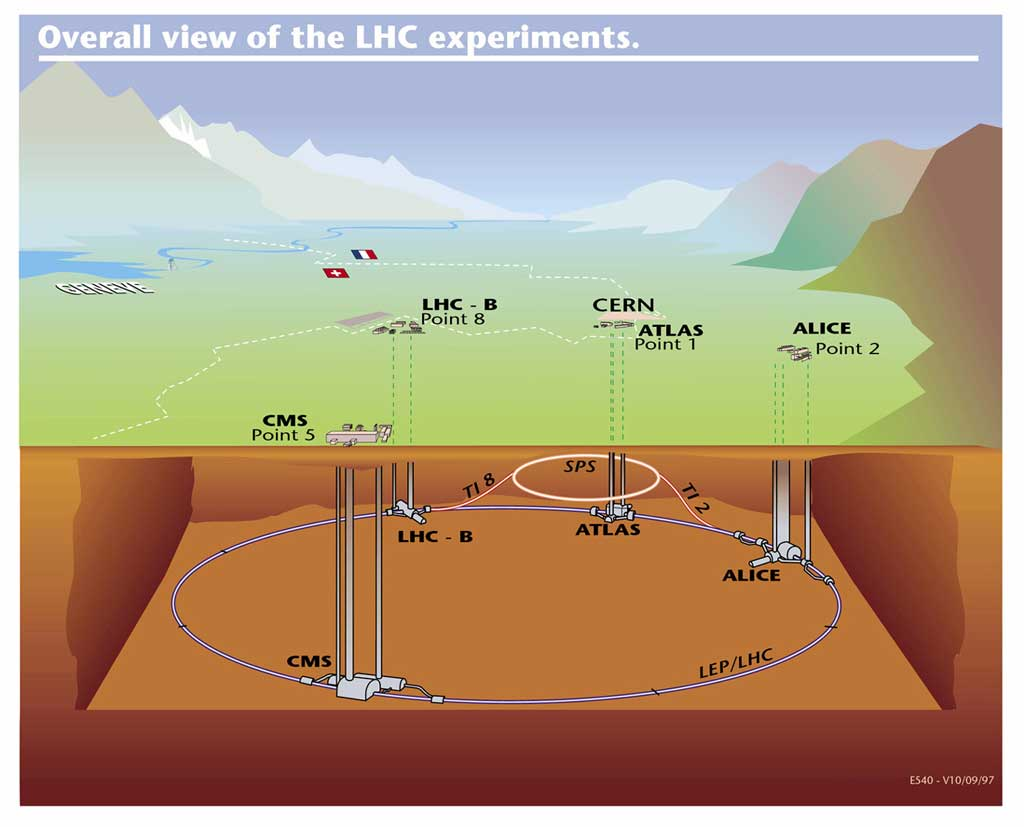
\includegraphics[width=\textwidth]{pics/lhc.jpg}
\caption{The LHC near Geneva at the Swiss-French border}
\end{figure}
    \end{column}
    \begin{column}{0.5\textwidth}
    Hosts four large experiments:
\begin{itemize}
  \item CMS/ATLAS - Multipuprose experiments with the main goal of probing $p--p$ collisions for direct search of new particles.
  \item ALICE - heavy ion detector
  \item LHC\textit{b} - Testing the Standard Model by confronting its predictions with precise measurements in CP violations and rare decays.
\end{itemize}
    \end{column}
  \end{columns}


\end{frame}


% section lhc (end)

\subsection{LHCb} % (fold)
\label{sec:lhcb}

\begin{frame}[c]\frametitle{LHC\textit{b}}
    
\begin{itemize}
  \item Studies decay containing $b$ and $\bar{b}$ quarks
  \item Single arm forward spectormeter
\end{itemize}

\begin{figure}
  \centering
  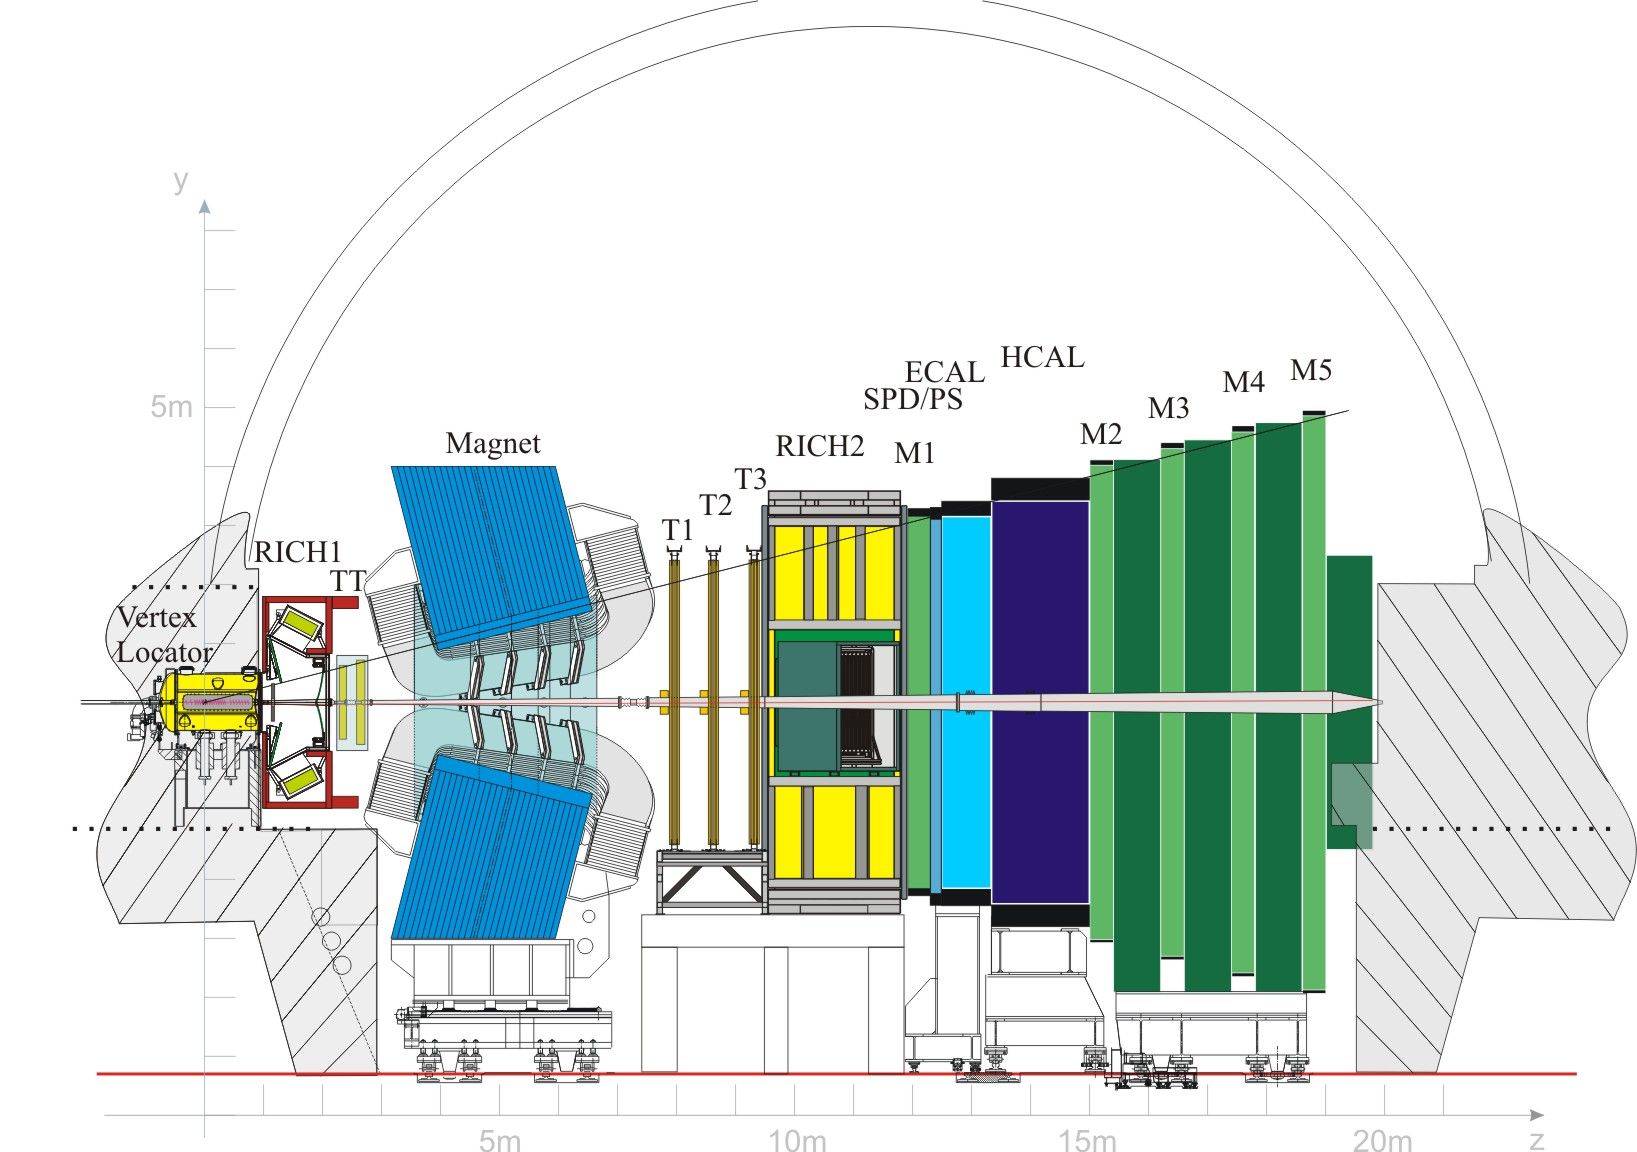
\includegraphics[width=0.7\textwidth]{pics/lhcb_detector.jpg}
  \caption{LHC\textit{b} detector}
  \label{fig:lhcb}
\end{figure}
\end{frame}
% section lhctextit (end)


\subsection{Cherenkov Radiation} % (fold)
\label{sub:cherenkov_radiation}

\begin{frame}[c,allowframebreaks]\frametitle{Cherenkov radiation}
    \begin{figure}
      \includegraphics[width=0.5\textheight]{pics/cherenkov_radiation.jpg}
      \caption{Cherenkov radiation in the Advanced Test Reactor of Arco, Idaho.}
    \end{figure}
\begin{columns}
  \begin{column}{0.5\textwidth}
    \begin{figure}[htbp]
  \centering
    \begin{tikzpicture}[scale=0.8]
      \draw (-1,0) -- (6,0);
      \draw (0,0) -- (1,2) -- (5,0);
      \draw (0,0) -- (1,-2) -- (5,0);
      \draw[->, red, thick] (-1,0) -- (-0.5,0);
      \draw (0.2,0)arc[radius=.3,start angle=0,end angle=45];
      \node [left] at (0.5,1) {\footnotesize$\dfrac{c}{n}t$};
      \node [below] at (2.5 ,0) {\footnotesize$\beta c t$};
      \node [right] at (0.2,0.2) {\footnotesize$\theta$};
      \foreach \x in {0,1,...,9} {
        \draw[->,blue, thick] (1.1 + \x*0.4, 2.1 - \x*0.2)  --+ (63.435:0.3);
        \draw[->,blue, thick] (1.1 + \x*0.4, -2.1 + \x*0.2) --+ (-63.435:0.3);
      }
    \end{tikzpicture}
  \caption{The geometry of the Cherenkov radiation}
  \label{fig:label}
\end{figure}
  \end{column}
  \begin{column}{0.5\textwidth}

    \begin{itemize}
      \item Particle travelling faster than speed of light in a medium
      \item $n$ is the refraction index of the radiator
      \item $\beta = \frac{v}{c}$ where $v$ is the speed of the particle and $c$ the speed of light
      \item Particle creates electro-magnetic shockwave
    \end{itemize}
  \end{column}
\end{columns}

\end{frame}

% subsection cherenkov_radiation (end)

\subsection{RICH Detector} % (fold)
\label{sec:rich_detector}

\begin{frame}[c]\frametitle{RICH detector}
\begin{columns}
      \begin{column}{0.4\textwidth}
      \begin{figure}
      \centering
         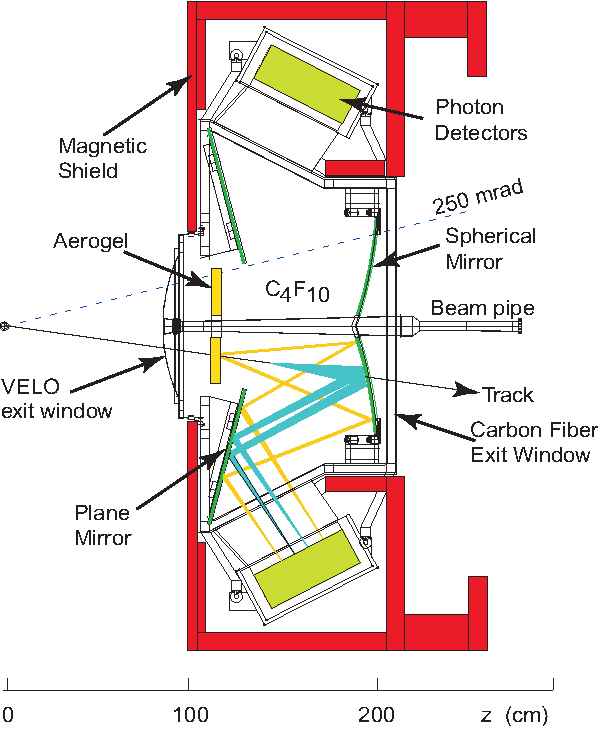
\includegraphics[width=\textwidth]{pics/rich1-2d.pdf}
         \caption{RICH-1 Detector}
      \end{figure}
    \end{column}%
    \begin{column}{0.5\textwidth}
      \begin{itemize}
        \item Placed in low magnetic region to avoid track bending
        \item Radiators for different momentum coverage
        \item Spherical mirrors for focusing light on flat mirror
        \item Hyprid photon detectors
      \end{itemize}
    \end{column}
\end{columns}


\end{frame}
% section rich_detector (end)


\subsection{Hough transform} % (fold)
\label{sub:linear_hough_transform}
\begin{frame}[c]
  \frametitle{Hough transform}


  \begin{itemize}
    \item Feature extraction technique.
    \item Used in image analysis, computer vision, digital image processing
    \item Find imperfect instances of objects (e.g. lines, circles)
    \item Voting procedure carried out in an accumulator space
  \end{itemize}
\end{frame}

\subsubsection{Linear Hough transform} % (fold)
\label{ssub:linear_hough_transform}

\begin{frame}[c,allowframebreaks]\frametitle{Linear Hough transform}
    
The Hough transform is a technique used to extract shapes (e.g. lines, circles) from images.
A linear function is often parametrized as:
\begin{equation}
  f(x) = mx + b
\end{equation}
If the line is perpendicular, $m = \infty$. This leads to an unbound parameters space so another representation of a line is needed.
\framebreak

Linear Hough transform uses an $r,\theta$ parametrizsation for a line

\begin{equation}
 r = x\cos(\theta) + y\sin(\theta)
\end{equation}

$r$ is the distance closest to the origin on the straight line.

\begin{figure}[ht]
  \centering
  \begin{tikzpicture}[scale=1.5]
    \draw[<->] (0,1.5) -- (0,0) -- (1.5,0);
    \node [left] at (0,1.5) {$y$};
    \node [below] at (1.5,0) {$x$};
    \draw[green,semithick] (0,1) -- (1,0);
    \draw[-> ,semithick] (0,0) -- (0.5, 0.5);
    \draw[semithick] (0.2,0) arc (0:45:0.2cm);
    \node[below] at (0.25,0.25) {\footnotesize$\theta$};
    \node[above] at (0.2,0.2) {\footnotesize$r$};
  \end{tikzpicture}
  \caption{$r\text{-}\theta$ parametrisation}
  \label{fig:rhotheta}
\end{figure}
\end{frame}

\begin{frame}[c,allowframebreaks,fragile]
  \frametitle{Linear Hough Transform}
  \framesubtitle{Example}
  \vspace*{\fill}
  \begin{figure}
  \centering
    \includegraphics[width=0.56\textwidth]{pics/Hough_transform_diagram}
  \end{figure}
    \vspace{\fill}

    \tiny \detokenize{By Mike1024 - http://en.wikipedia.org/wiki/Image:Hough_transform_diagram.png, Public Domain, https://commons.wikimedia.org/w/index.php?curid=4451739}

\framebreak
\vspace*{\fill}
  \begin{figure}
    \includegraphics[width=0.4\textwidth]{pics/Hough_space_plot_example.png}
    \caption{Accumulator space for the linear Hough transform}
  \end{figure}

  \vspace{\fill}
  \tiny\detokenize{By Mike1024 - the English language Wikipedia (log), Public Domain, https://commons.wikimedia.org/w/index.php?curid=4451726}
  
\end{frame}

% subsubsection linear_hough_transform (end)

\subsubsection{Circle Hough transform} % (fold)
\label{ssub:circle_hough_transform}

\begin{frame}[c]\frametitle{Circle Hough transform}

Instead of a line a circle has to be found. Condition that a point ($x,y$) lies on a circle with
center coordinate ($x_c,y_c$) and radius $r$:

\begin{equation}
  (x-x_c)^2 + (y-y_c)^2 - r_c = 0
\end{equation}

Depending on what information is given the parameter space of the circle Hough Transform changes.
\begin{itemize}
  \item Center is known: 1D parameter space
  \item Radius is known: 2D parameter space
  \item Both unknown: 3D parameter space
\end{itemize}
\end{frame}

\begin{frame}
  \frametitle{Circle Hough transform} 
  Instead of points on a line there are now points on a circle (and maybe some background hits).
  \begin{figure}
    \includegraphics[width=0.5\textwidth]{pics/points_on_circle.pdf}
  \end{figure}
\end{frame}
% subsubsection circle_hough_transform (end)
% subsection linear_hough_transform (end)

\section{Methods} % (fold)
\label{sec:methods}

\subsection{1D Hough transform} % (fold)
\label{sub:1d_hough_transform}

\begin{frame}[c,allowframebreaks]\frametitle{1D Hough transform}
The center coordinates ($x_c,y_c$) are known. Find the radius $r$ to this circle.

Using a scoring function to measure for which radius a given point lies closest on the circle with center ($x_c, y_c$).

\begin{equation}
  \eta(r) = (x-x_c)^2 + (y-y_c)^2 - r
\end{equation}

Define an array of $r$ values from $0-0.5$

\begin{figure}
  $r$ = \begin{tikzpicture}
  \draw (0,-0.3) -- (5,-0.3);
  \foreach \x in {0,1,...,5} {
  \draw (\x,-0.3) -- (\x,0.1);
  }

  \def\numberlist{0.1,0.2,0.3,0.4,0.5}
  \def\coordlist{0.5,1.5,...,4.5}
   \foreach \x [count=\c,evaluate=\c as \y using {{\numberlist}[\c-1]}]  in \coordlist {
  \node at (\x,0) {$\y$};
  }
\end{tikzpicture}
\end{figure}
\framebreak

Need a way to reliably score the different radiuses.

\begin{equation}
  w(\eta) = \frac{1}{\sqrt{2\pi}\sigma}\exp\left( \frac{-\eta^2}{2\sigma^2}\right)
\end{equation}

There is a maximum for $w(\eta)$ if $\eta=0$.

\begin{figure}[ht]
\centering
  \begin{tikzpicture}[scale=0.4]
    \begin{axis}[
    axis lines = center,
    ymin=0, ymax=45,
    xlabel = $\eta$,
    scaled x ticks = false,
    % x tick label style={},
    x label style={at={(axis description cs:1.05,0.0)},anchor=north},{/pgf/number format/fixed},
    ylabel = $\omega(\eta)$,
    legend style={at={(0.2,0.7)},anchor=east},
    legend cell align=left,
    ]
    \addplot [
    domain=-0.05:0.05, 
    color=red,
    samples=200,
    ]
    { 1/(sqrt(2*pi)*0.01)*exp(-x^2/(2*0.01^2))};
    \addplot [
    domain=-0.05:0.05, 
    color=blue,
    samples=200,
    ]
    { 1/(sqrt(2*pi)*2*0.01)*exp(-x^2/(2*(2*0.01)^2))};
    \addlegendentry{$\sigma=0.01$}
    \addlegendentry{$\sigma=0.02$}
    \end{axis}

  \end{tikzpicture}
  \label{fig:gauss}
\end{figure}
\framebreak

\begin{figure}[tb]
  \centering
  \includegraphics[width=0.8\textwidth]{sim_pics/1D_HT/radius_scores_forpresentation_1}
  \caption[Graph visualisation of a 1D radius histogram]{Visualisation of a 1D radius score histogram. The peak between $0.2$ 
  and $0.3$ has by far the highest score and the bin
  position of the peak is the radius candidate for a given circle center ($c_x, c_y$)}
  \label{fig:1d_ht_radius_score}
\end{figure}
\end{frame}

% subsection 1d_hough_transform (end)

\subsection{2D Hough transform} % (fold)
\label{sub:2d_hough_transform}

\begin{frame}[c]\frametitle{2D Hough transform}
    


\end{frame}

% subsection 2d_hough_transform (end)

\subsection{3D Hough transform} % (fold)
\label{sub:3d_hough_transform}

\begin{frame}[c]\frametitle{3D Hough transform}
    


\end{frame}

% subsection 3d_hough_transform (end)

\subsection{Combinatorial Hough transform} % (fold)
\label{sub:combinatorial_hough_transform}

\begin{frame}[c]\frametitle{Combinatorial Hough transform}
    


\end{frame}

% subsection combinatorial_hough_transform (end)

% section methods (end)

\section{Results} % (fold)
\label{sec:results}

\begin{frame}[c]\frametitle{Results}
    


\end{frame}

\subsection{Conventional Hough transform results} % (fold)
\label{sub:conventional_hough_transform_results}

% subsection conventional_hough_transform_results (end)

\subsection{Combinatorial triplet results} % (fold)
\label{sub:combinatorial_triplet_results}

% subsection combinatorial_triplet_results (end)
% section results (end)

\section{Conclusion and Outlook} % (fold)
\label{sec:conclusion_and_outlook}

\begin{frame}[c]\frametitle{Conclusion and Outlook}
    


\end{frame}

% section conclusion_and_outlook (end)

\end{document}